\documentclass{itkmitlproject}

\usepackage{afterpage}
\usepackage{graphicx,amsmath,latexsym,amssymb,amsthm}
\usepackage{indentfirst}
\usepackage{hyperref}
\usepackage{hyphenat}
\usepackage[numbers,square]{natbib}
\usepackage{everyshi}

% \useEnglish
\useThai

\graphicspath{ {images/} }
\makeatletter
% \patchcmd{<cmd>}{<search>}{<replace>}{<succes>}{<failure>}
\patchcmd{\@chapter}{\addtocontents{lof}{\protect\addvspace{10\p@}}}{}{}{}% LoF
\patchcmd{\@chapter}{\addtocontents{lot}{\protect\addvspace{10\p@}}}{}{}{}% LoT
\def\bibindent{2.3em}
\let\old@biblabel\@biblabel
\def\@biblabel#1{\old@biblabel{#1}\kern\bibindent}
\let\old@bibitem\bibitem
\def\bibitem#1{\old@bibitem{#1}\leavevmode\kern-\bibindent}

\def\@biblioProblem{%
   \parindent \z@ \raggedright
     \normalfont
     \interlinepenalty\@M
     \centering
     \LARGE \bfseries \bibname\space(\continuename) \par\nobreak
     \vskip1.15em
}

\gdef\@cont@heading{%
    \@biblioProblem
    %\@afterheading
}

\makeatother

%1. Your thesis title (THAI)
\newcommand{\ThesisTitle}{ชื่อโปรเจ็กต์จบ}
%2. Your thesis title (ENG)
\newcommand{\ThesisTitleENG}{Project name (English)}
%3. Author name
\newcommand{\Author}{ชื่อ นามสกุล}
%4. Author name ENG
\newcommand{\AuthorENG}{Name Surname}
%5. Author student ID
\newcommand{\SId}{59070000}
%6. Author 2 name
\newcommand{\AuthorTwo}{ชื่อ นามสกุล}
%7. Author 2 name ENG
\newcommand{\AuthorTwoENG}{Name Surname}
%8. Author 2 student ID
\newcommand{\SIdTwo}{59070000}
%9. Advisor name
\newcommand{\Advisor}{ชื่อที่ปรึกษา}
%10. Advisor name ENG
\newcommand{\AdvisorENG}{Advisor Name}
%11. ภาคเรียนที่
\newcommand{\Sem}{1}
%12. ปีการศึกษา พ.ศ.
\newcommand{\AcaY}{2562}
%13. ปีการศึกษา ค.ศ.
\newcommand{\AcaYAD}{2019}
%14. วันส่งรายงาน
\newcommand{\SubD}{10 พฤศจิกายน พ.ศ. 2561}
%15. Copyright year (AD)
\newcommand{\CopyrightYAD}{2020}

\begin{document}
    \frontmatter
    \lhead{}\rhead{}\chead{}\lfoot{}\cfoot{\thepage}\rfoot{}
    \makecover
    \makeinnercover
    \makeengcover
    \makecopyrightcover
    \makethesiscert
    \makeprojectcert

    % Setting margin for page numbering on frontmatter
    \newgeometry{top=1in, bottom=1in, left=1.5in, right=1in, includefoot}
    \setcounter{page}{1}
    \pagenumbering{Roman}

    \makeabstract{
        บทคัดย่อ
    }

    \makeabstracteng{
        Abstract eng
    }

    \makeack

    \newpage
    \addcontentsline{toc}{chapter}{\contentsname}
    \tableofcontents

    \newpage
    \addcontentsline{toc}{chapter}{\listtablename}
    \listoftables

    \newpage
    \addcontentsline{toc}{chapter}{\listfigurename}
    \listoffigures

    % Reset frontmatter page numbering margin, back to original margin from class file
    \restoregeometry

    \mainmatter
    \lhead{}\rhead{\thepage}\chead{}\lfoot{}\cfoot{}\rfoot{}

    \chapter{บทนำ}
\label{chapter:introduction}

\section{การเขียนรายงาน}

นักศึกษาจะต้องเขียนรายงานให้ถูกต้องตามรูปแบบที่กำหนด นอกเหนือจากรูปแบบของรายงานแล้ว นักศึกษาควรให้ความสำคัญกับการใช้ภาษาและการจัดเรียงหัวข้อที่ต่อเนื่อง รวมถึงการอธิบายที่กระชับแต่ได้ใจความ อันเป็นลักษณะของการเขียนรายงานทางวิชาการที่ดี คำศัพท์ต่าง ๆ ต้องเขียนให้ถูกตามศัพท์บัญญัติราชบัณฑิตยสถาน ซึ่งสามารถตรวจสอบได้ที่ \url{http://www.royin.go.th/?page_id=15521}

หากมีการอ้างอิงข้อมูลจากแหล่งอื่นๆ นักศึกษาสามารถทำได้โดยมี 2 วิธี ดังนี้
\begin{enumerate}
    \item ต้องเขียนด้วยสำนวนของตนเอง และอ้างอิงถึงแหล่งที่มาของความคิดนั้นๆ
    \item ถ้าคัดลอกข้อความใดๆ มาจะต้องทำการอ้างอิงพร้อมใส่เครื่องหมายอัญประกาศคร่อมประโยคนั้นๆอนึ่งการคัดลอกวิธีนี้สามารถทำได้โดยไม่เกิน 15\% ของจำนวนข้อความทั้งหมดของเล่มรายงาน
\end{enumerate}

\textbf{หมายเหตุ ถ้ากรรมการตรวจพบการคัดลอกโดยไม่ตรงตามข้อกำหนด นักศึกษาจะถูกทำโทษโดยการได้รับผลคะแนนเป็น F ทันที}

\section{รูปแบบรายงาน}
\subsection{ส่วนประกอบของรายงานและการเรียงลำดับ}
\begin{itemize}
    \item \textbf{ปกนอก} (ภาษาไทย) ให้ใช้กระดาษขาวลักษณะเดียวกับที่ใช้พิมพ์ตัวรายงานเป็นปกนอก พร้อมพิมพ์ชื่อเรื่อง ชื่อนักศึกษา ชื่ออาจารย์ที่ปรึกษา รหัสประจำตัว และชื่อวิชา (ไม่ต้องใส่คำนำหน้าชื่อ อาจารย์ที่ปรึกษาใช้ตัวอักษรขนาด 20 ตัวหนา ส่วนล่างตั้งแต่ ``ปริญญานิพนธ์นี้... ''ใช้ตัวอักษรขนาด 18 ตัวหนา) ดูตัวอย่างในภาคผนวก
    \item \textbf{ปกใน} (ภาษาอังกฤษ) ใช้ตัวพิมพ์ใหญ่ทั้งหมด โดยมีขนาด 20 ตัวหนา ส่วนล่างตั้งแต่ ``A PROJECT SUBMITTED IN PARTIAL... '' ใช้ตัวอักษรขนาด 18 ตัวหนา
    \item \textbf{Copyright} อยู่ส่วนล่างของหน้ากระดาษด้านซ้าย ใช้ตัวอักษรขนาด 18ตัวหนา (แสดงปีที่ตีพิมพ์ปัจจุบัน)
    \item \textbf{ใบรับรองปริญญานิพนธ์} ตั้งแต่คำว่า ใบรับรองปริญญานิพนธ์... จนถึงสถาบันฯ (3 บรรทัดแรก) ใช้ขนาดอักษร 24 ตัวหนา ส่วนคำว่า เรื่อง ภาษาไทยและภาษาอังกฤษ (ตัวอักษรพิมพ์ใหญ่) และผู้จัดทำ ขนาดตัวอักษร 20 หนา ชื่ออาจารย์ที่ปรึกษาและที่ปรึกษาร่วม (ถ้ามี) ขนาดอักษร 18 หนา
    \item \textbf{ใบรับรองโครงงาน} (เฉพาะรายงานต้นฉบับและรายงานฉบับสมบูรณ์) ใบรับรองการตรวจสอบและอนุมัติรายงาน ตั้งแต่คำว่า ``ใบรับรองโครงงาน... '' จนถึงรหัสประจำตัว ใช้ตัวอักษรขนาด 20 ตัวหนาในส่วนของคำว่า ``ขอรับรองว่า... '' ใช้ตัวอักษรขนาด 16 ตัวหนา และในส่วนของคำว่า ``อาจารย์ที่ปรึกษา/กรรมการ.. '' ใช้ตัวอักษรขนาด 16 ตัวหนา
    \item \textbf{บทคัดย่อภาษาไทย} ประกอบด้วยชื่อหัวข้อโครงงาน ชื่อนักศึกษา ชื่ออาจารย์ที่ปรึกษา ระดับการศึกษา และปีการศึกษา ดังตัวอย่างในภาคผนวก (คำว่า ``บทคัดย่อ'' ใช้ตัวอักษรขนาด 24 ตัวหนา)
    \item \textbf{บทคัดย่อภาษาอังกฤษ} มีรูปแบบเช่นเดียวกับบทคัดย่อภาษาไทยดังตัวอย่างในภาคผนวก (คำว่า ``ABSTRACT'' ใช้ ตัวอักษรขนาด 24ตัวหนา)
    \item \textbf{กิตติกรรมประกาศ} ใช้กล่าวขอบคุณบุคคลที่มีส่วนช่วยเหลือในการศึกษา (คำว่า ``กิตติกรรมประกาศ'' ใช้ตัวอักษรขนาด 24 ตัวหนา)
    \item \textbf{สารบัญ} ซึ่งแสดงเลขที่หน้าของ บทคัดย่อ สารบัญ กิตติกรรมประกาศ บทต่างๆ ในส่วนของเนื้อหา บรรณานุกรม ฯลฯ มีคำว่า ``สารบัญ'' ตรงกลางหน้าใช้ตัวอักษรขนาด 24 ตัวหนาถ้ามีต่อหน้า 2 มีคำว่า ``สารบัญ (ต่อ)
    \item \textbf{สารบัญรูป/สารบัญตาราง} อาจมีหรือไม่ก็ได้ขึ้นอยู่กับเนื้อหาภายในเล่ม ถ้ามีจะอยู่ถัดจากหน้าสารบัญ คำว่า ``สารบัญรูป'' ใช้ตัวอักษรขนาด 24 ตัวหนาถ้ามีต่อหน้า 2 มีคำว่า ``สารบัญรูป (ต่อ) โดยมีรูปแบบเดียวสารบัญ
    \item \textbf{คำนิยามศัพท์} อาจมีหรือไม่ก็ได้แล้วแต่ความเหมาะสม คือ การอธิบายคำย่อต่างๆ ที่อยู่ในรายงาน
    \item \textbf{เนื้อหา} ประกอบไปด้วย (1) บทนำ (2) การทบทวนวรรณกรรมที่เกี่ยวข้อง (3) วิธีการดำเนินการวิจัย (4) ผลการทดลอง/ระบบต้นแบบ (5) วิเคราะห์และสรุปผล
    \item \textbf{บรรณานุกรม} รายชื่อหนังสือหรือเอกสารอ้างอิงที่นำมาใช้ในการเขียนรายงาน
    \item \textbf{ภาคผนวก} เป็นส่วนที่ใช้ในการให้ข้อมูลเสริมเพื่อให้ผู้อ่านมีความเข้าใจเนื้อหาหลักของโครงงานได้ดีขึ้น หรืออาจเป็นส่วนที่รวบรวมข้อมูลที่ถูกอ้างอิงถึงในส่วนของเนื้อหาหลักก็ได้ ใช้ตัวอักษรขนาด 24 ตัวหนา อยู่กึ่งกลางหน้ากระดาษ (อาจมีหรือไม่มีก็ได้ แล้วแต่ความเหมาะสม)
    \item \textbf{ประวัติผู้เขียนข้อมูลเกี่ยวกับผู้เขียน} โดยประกอบด้วย คำนำหน้าชื่อ นาย/นาง/นางสาว ยศ ฐานันดรศักดิ์ สมณศักดิ์ ราชทินนาม ตามด้วยชื่อ วัน เดือน ปี และสถานที่เกิด ประวัติการศึกษาและประวัติการทำงาน (คำว่า ``ประวัติผู้เขียน'' ใช้ตัวอักษรขนาด 24 ตัวหนา)
\end{itemize}

\subsection{การเว้นระยะห่างจากริมกระดาษ}
    ได้ถูกแสดงดังรูปที่ \ref{fig:page-padding}
    \begin{enumerate}
        \item หน้าบทคัดย่อถึงหน้าสารบัญ
        \item หน้าแรกของแต่ละบท
        \item หน้าปกติ
    \end{enumerate}

    \begin{figure}[ht]
        \centering
        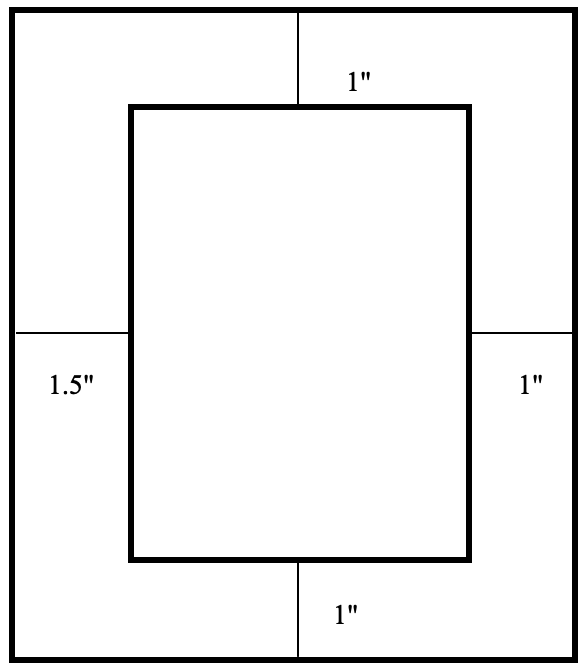
\includegraphics[width=110mm,scale=0.6]{page-padding.png}
        \caption{การเว้นระยะห่างจากริมกระดาษ}
        \label{fig:page-padding}
    \end{figure}

\subsection{เลขที่หน้า}

\begin{enumerate}
    \item ตั้งแต่บทคัดย่อถึงสารบัญ ให้ใช้ตัวอักษรโรมัน I, II, III, IV, … แสดงเลขหน้า โดยพิมพ์ไว้ตรงกลางส่วนล่างของหน้า ห่างจากด้านล่าง 1 นิ้ว
    \item ในส่วนของเนื้อหา (บทที่ 1เป็นต้นไป) ให้ใช้ตัวเลขอารบิค 1, 2, 3, 4, … แสดงเลขหน้า โดยพิมพ์ไว้ด้านขวามือห่างจากขอบบน 0.5 นิ้ว และห่างจากริมขอบกระดาษด้านขวามือ 1 นิ้ว หน้าแรกของแต่ละบทไม่ต้องมีเลขหน้าปรากฏ แต่นับรวมเป็น 1 หน้า
\end{enumerate}

\subsection{การพิมพ์ตาราง}

ให้แทรกปนไปในแต่ละบทของเนื้อเรื่องที่มีความสัมพันธ์ โดยพิมพ์"ตารางที่"อยู่ด้านบน (ใช้อักษร ตัวหนา) ชิดขอบซ้ายของหน้ากระดาษ ตามด้วยชื่อตาราง (ใช้ตัวอักษรปกติ) ถ้าชื่อตารางมีความยาวเกินกว่า 1 บรรทัด ให้พิมพ์บรรทัดล่าง เริ่มพิมพ์ตรงกับตัวอักษรตัวแรกของคำบรรยายตาราง พิมพ์ตารางโดยไม่ต้องเว้นบรรทัดจากชื่อตาราง เมื่อพิมพ์ตารางจบแล้วให้เว้นไว้ 1บรรทัดก่อนการพิมพ์ปกติหากตารางไม่จบในหน้าเดียวให้ขึ้นหน้าใหม่ โดยพิมพ์คำว่า ตารางที่ ........ (ต่อ) แล้วตามด้วยชื่อตาราง

\subsection{การเรียงเลขตาราง}

ให้เรียงไปตามบท เช่น ในบทที่ 1 ให้พิมพ์ตารางที่ 1.1, ตารางที่ 1.2 ในบทที่ 2 ให้พิมพ์ ตารางที่ 2.1, ตารางที่ 2.2 เป็นต้น

\subsection{การพิมพ์รูป}

ให้เว้น 1 บรรทัดก่อนจัดวางรูปภาพกลางหน้ากระดาษ และใส่คำว่า "รูปที่……" โดยใช้ตัวอักษร ตัวหนา ตามด้วยคำบรรยายไว้กึ่งกลาง ใต้ภาพ ถ้าคำบรรยายเกิน 1บรรทัดให้พิมพ์บรรทัดล่างเริ่มพิมพ์ตรงกับอักษรตัวแรกของคำบรรยายภาพ และเว้น 1 บรรทัด ก่อนพิมพ์ปกติต่อไป การเรียงหมายเลขรูปที่ ให้เรียงไปตามบทเช่นในบทที่ 1 ให้พิมพ์รูปที่ 1.1, รูปที่ 1.2 ในบทที่ 1 ให้พิมพ์ รูปที่ 2.1, รูปที่ 2.2 เป็นต้น

\subsection{การพิมพ์เครื่องหมายวรรคตอน}
\begin{itemize}
    \item เครื่องหมายมหัพภาค	(.) 	ให้พิมพ์	เว้นระยะ 	2 อักษร
    \item เครื่องหมายจุลภาค	(,)	ให้พิมพ์เว้นระยะ 	1 ช่วงตัวอักษร
    \item เครื่องหมายอัฒภาค	(;)	ให้พิมพ์เว้นระยะ 	1 ช่วงตัวอักษร
    \item เครื่องหมายมหัพภาคคู่	(:)	ให้พิมพ์เว้นระยะ	1 ช่วงตัวอักษร
    \item เครื่องหมายอัญประกาศ	(“  ”)ให้พิมพ์เว้นระยะ 		1 ช่วงตัวอักษร
\end{itemize}


\subsection{การเขียนบรรณานุกรม}

เป็นส่วนที่แสดงถึงการศึกษาค้นคว้าวิจัยของผู้เขียนว่า มีความสมบูรณ์กว้างขวาง ลึกซึ้ง ทันสมัยน่าเชื่อถือมากน้อยเพียงใด โดยทั่วไป คำว่า บรรณานุกรม รวบรวมรายการเอกสารสิ่งพิมพ์ โสตทัศน์ สื่ออิเล็กทรอนิกส์ ที่ผู้เขียนศึกษาค้นคว้าทั้งหมด แม้ว่าจะไม่ได้คัดลอกข้อความมา ส่วนคำว่า เอกสารอ้างอิงนิยมใช้กับรายการเอกสาร สิ่งพิมพ์ โสตทัศน์ เฉพาะที่คัดลอกและยกมาอ้างอิงในเนื้อหา
บรรณานุกรมเป็นส่วนประกอบสำคัญส่วนหนึ่งของการผลิตสิ่งพิมพ์โดยเฉพาะสิ่งพิมพ์ประเภทตำราหรือหนังสือเรียน และเอกสารประกอบการสอน เพราะเป็นส่วนที่ระบุถึงหนังสือและเอกสารต่าง ๆ ตลอดจนการสัมภาษณ์ที่ผู้เขียนใช้เป็นแหล่งข้อมูลในการอ้างอิง

\textbf{ตัวอย่างการแทรกบรรณานุกรมที่อ้างอิงถึง}

เนื่องจากในการถอดรหัสในเชิงความถี่นี้จะต้องใช้การแปลงและแปลงกลับเป็นส่วนสำคัญ \cite{schroffFaceNetUnifiedEmbedding2015} นอกเหนือไปจากการคำนวณอื่นๆ การแปลงและการแปลงกลับจะต้องใช้การคำนวณเป็นจำนวนมากจึงมีการนำวิธีการตัวประกอบปฐม (Prime factor Algorithm) มาใช้เพื่อลดจำนวนการคำนวณลงโดยใช้ร่วมกับวิธีการแปลงข้อมูลจำนวนน้อยๆ (Short Length Algorithm) \cite{sagonas300FacesIntheWild2013} ในแง่ของการนำวิธีการดังกล่าวไปใช้งานจริงซึ่งจะต้องพิจารณา
\cite{chungEmpiricalEvaluationGated2014}
\cite{fernandez-lopezSurveyAutomaticLipreading2018}
\cite{sunHumanActionRecognition2015}
\cite{wangDeepFaceRecognition2018}
\cite{chungEmpiricalEvaluationGated2014}
\cite{sagonasSemiautomaticMethodologyFacial2013}
\cite{fungEndToEndLowResourceLipReading2018}
\cite{petridisVisualOnlyRecognitionNormal2018}
\cite{tranCloserLookSpatiotemporal2017}
\cite{xiaogangwangBoostedMultitaskLearning2009}
\cite{nvidiaTensorFlowDeterminism}

    \chapter{แนวคิด ทฤษฎีและงานวิจัยที่เกี่ยวข้อง}
\label{chapter:related-theory}

บทที่สอง
    \chapter{วิธีการดำเนินการวิจัย}
\label{chapter:experiment}

บทที่สาม

    \chapter{ผลการทดลอง}
\label{chapter:result}

ผลลัพธ์การทดสอบประสิทธิภาพในวิธีการใหม่ของเราและเปรียบเทียบกับงานวิจัยอื่น ๆ ที่เกี่ยวข้อง แสดงในตารางที่~\ref{Table:ExperimentalResults} จากตารางดังกล่าว วิธีการของเราได้รับ F-measure สูงที่สุด ที่ 0.506 ซึ่งแสดงให้เห็นชัดเจนว่าวิธีการของเรามีประสิทธิภาพดีกว่าวิธีการ SWT ต้นฉบับ~\cite{5540041} ยิ่งไปกว่านั้นวิธีการของเรายังได้รับ F-meaure ที่มากกว่าวิธีการ BG+ImN~\cite{7532890} และ BG+I2V~\cite{7532890} ซึ่งทั้งสองวิธีนี้ใช้เทคนิค Deep Learning เป็นส่วนหนึ่งในการตรวจหาข้อความในภาพ อย่างไรก็ดีค่า Precision และ Recall สูงสุดของการทดลองนี้อยู่ที่ 0.715 และ 0.481 เป็นของ BG+I2V และ BG+ImN ตามลำดับ สำหรับตัวอย่างพื้นที่ของข้อความที่วิธีการใหม่ของเราตรวจพบถูกแสดงในภาพ~\ref{Fig:ExampleResult}

\begin{table}[!h]    
    \centering
    \begin{tabular}{lccc}
        \hline
        Method & Precision & Recall & F-measure \\ \hline \hline
        STD~\cite{6628665} & 0.165 & 0.051 & 0.078 \\
        SBD~\cite{6761596} & 0.180 & 0.102 & 0.130 \\
        TLD~\cite{rigaud:hal-00841492} & 0.095 & 0.095 & 0.095 \\
        BG + ImN~\cite{7532890} & 0.451 & \textbf{0.481} & 0.466 \\
        BG + I2V~\cite{7532890} & \textbf{0.715} & 0.191 & 0.301 \\
        Baseline~\cite{5540041} & 0.068     & 0.336 & 0.113 \\
        วิธีการของเรา & 0.564     & 0.458 & \textbf{0.506} \\ \hline
    \end{tabular}
    \caption{ตารางแสดงการเปรียบเทียบประสิทธิภาพของวิธีการใหม่ของเราร่วมกับวิธีการอื่น ๆ ที่เกี่ยวข้อง}
    \label{Table:ExperimentalResults}
\end{table}


\begin{figure}[!h]
    \centering
    \subfigure[]{
        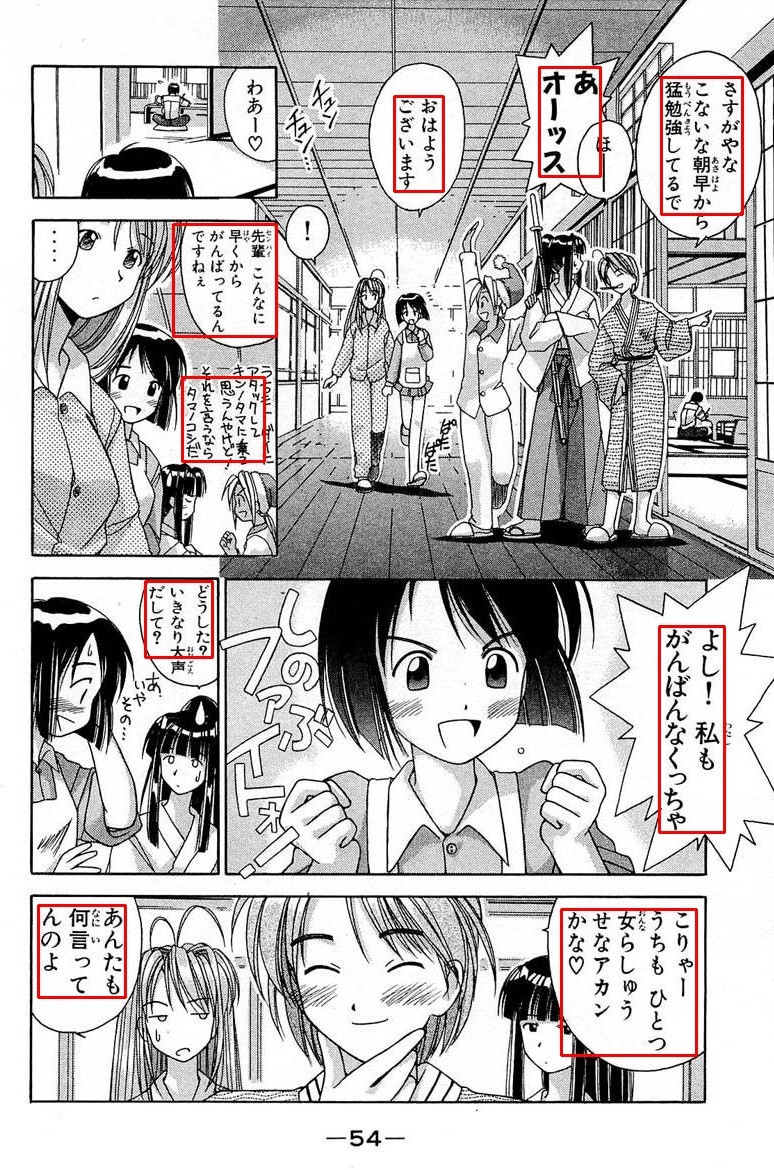
\includegraphics[width=0.45\textwidth]{images/result1.jpg}  
    }
    \subfigure[]{
        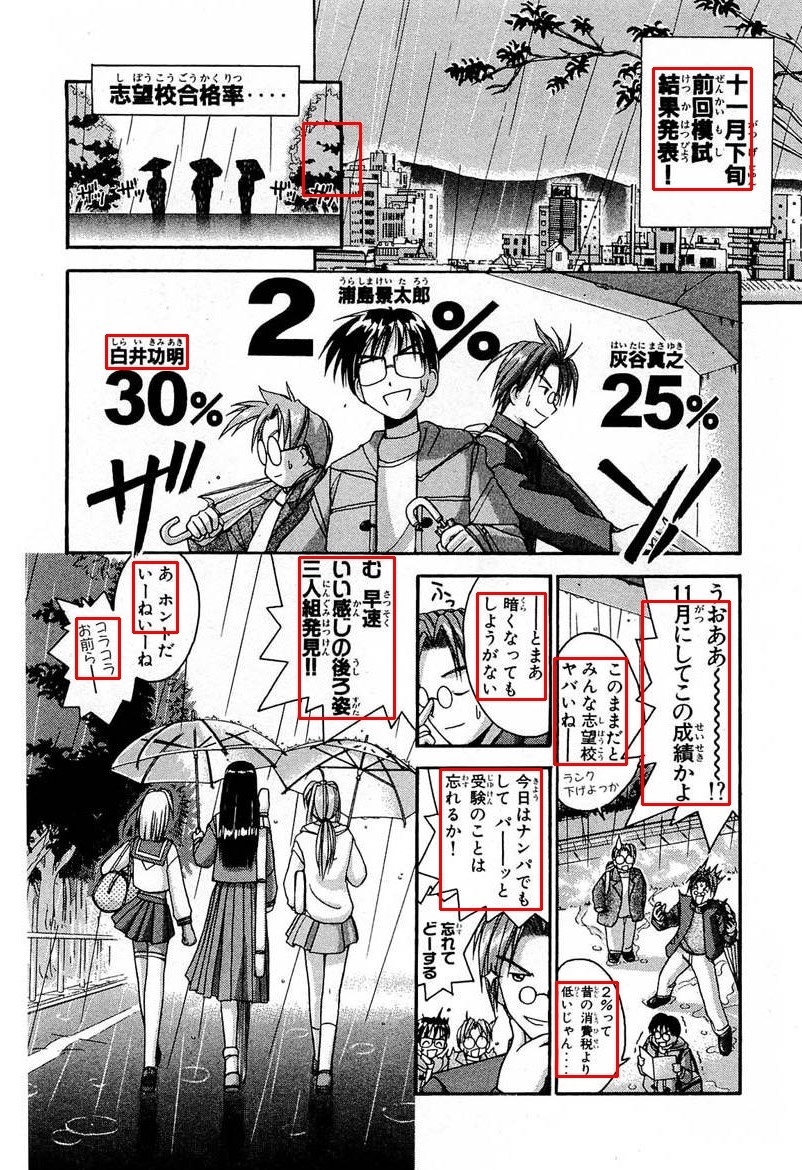
\includegraphics[width=0.45\textwidth]{images/result2.jpg}  
    }
    \subfigure[]{
        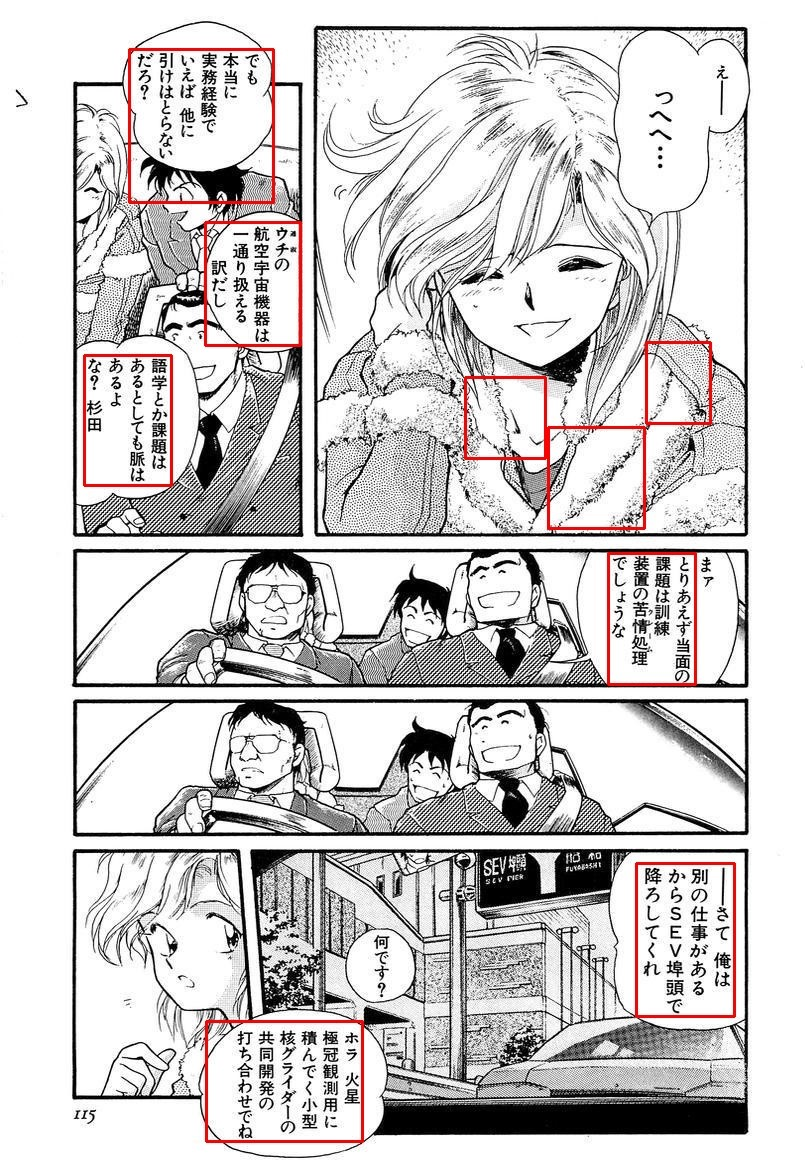
\includegraphics[width=0.45\textwidth]{images/result3.jpg}  
    }
    \subfigure[]{
        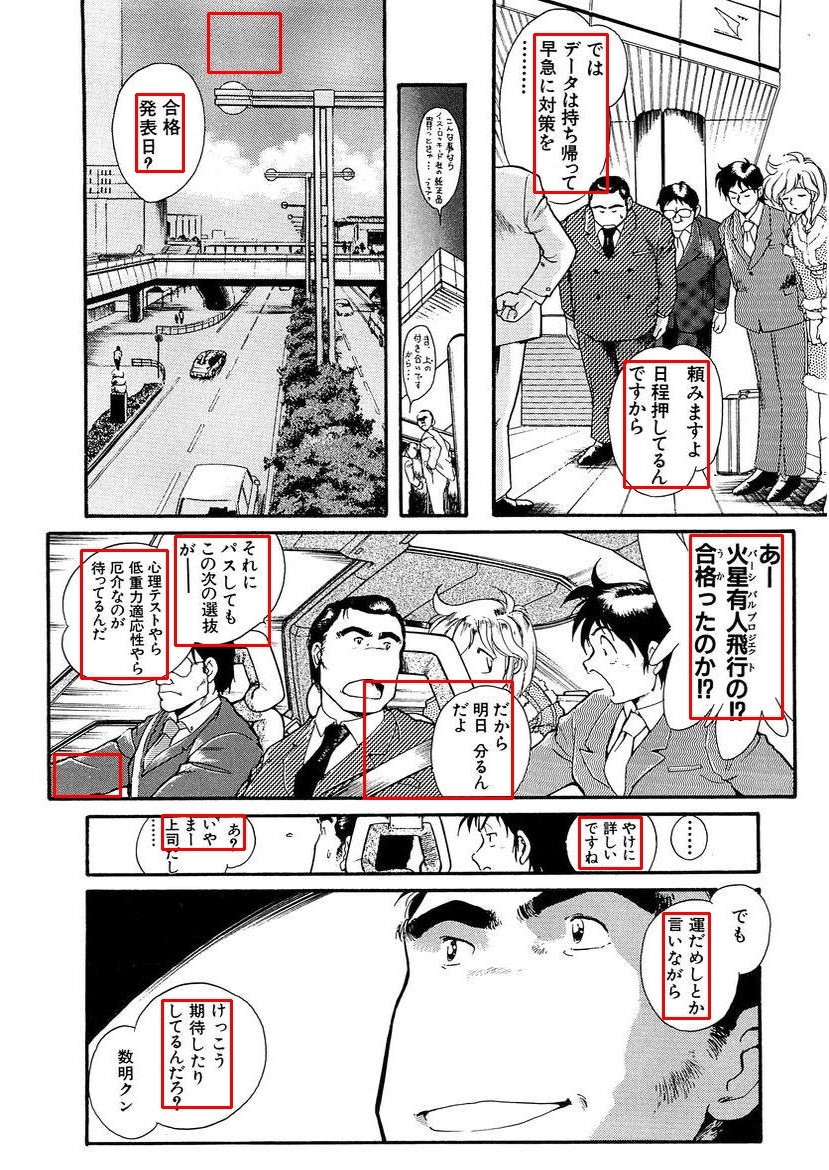
\includegraphics[width=0.45\textwidth]{images/result4.jpg}  
    }
    \caption{ตัวอย่างขอบเขตข้อความที่วิธีการของเราตรวจพบ (ก--ข) Love Hina \copyright Ken Akamatsu และ (ค--ง) Eva Lady \copyright Miyone Shi}
    \label{Fig:ExampleResult}
\end{figure}

เป็นที่น่าสนใจอย่างมากที่วิธีการของเราสามารถทำงานได้ดีกว่าเทคนิค Deep Learning ทั้งสองวิธี สมมติฐานแรกคือ BG+ImN นั้นใช้ ImageNet Classification Model~\cite{Krizhevsky} ซึ่งถูกเทรนบนภาพถ่ายของวัตถุจริง อย่างไรก็ดีภาพวาดมังงะของวัตถุต่าง ๆ นั้นมีความแตกต่างจากภาพวัตถุจริงอย่างชัดเจนซึ่ง ณ จุดนี้ทำให้วิธีการนี้ไม่สามารถทำงานได้เต็มประสิทธิภาพ อีกวิธีการที่ใช้ Deep Learning คือ BG+I2V ถึงแม้ว่าวิธีการนี้จะได้รับ Precision สูงที่สุดในการทดลองของเราแต่คะแนน Recal นั้นต่ำกว่าทั้ง BG+ImN และวิธีการของเรา วิธีการนี้ใช้โมเดล Illustration2Vec~\cite{Saito:2015:ISV:2820903.2820907} เป็นโมเดลสำหรับคัดแยกข้อความจากวัตถุอื่น ๆ ที่ปรากฎในภาพมังงะ ส่วนของโมเดลนั้นถูกเทรนบนภาพวาด Anime (ภาพการ์ตูนแบบญี่ปุ่น) และภาพมังงะจากหลากหลายแหล่งอันประกอบไปด้วย Danbooru และ Safebooru ซึ่งมีลักษณะงานคล้ายกับข้อมูลที่เราใช้ทดสอบในวิธีการของเรา แต่โมเดลนี้ถูกออกแบบมาเพื่อการทำนายป้ายกำกับ (Tag Prediction) และค้นหาภาพที่คล้ายคลึงกัน ดังนั้นการเลือกใช้วิธีการที่ไม่ต้องลักษณะงานโดยตรงในลักษณะนี้จึงอาจเป็นเหตุผลว่าทำไมโมเดลนี้จึงไมมีประสิทธิภาพเท่าที่ควรในการทดลองนี้

    \chapter{บทสรุป}
\label{chapter:conclusion}

บทที่ห้า


    \clearpage
    \addcontentsline{toc}{chapter}{\bibname}
    \bibliographystyle{IEEEtran}

    \makeatletter
    \EveryShipout{%
    \ifdim\pagetotal>\pagegoal% There is content overflow on this page % Bib
            \aftergroup\@cont@heading
    \fi%
    }
    \makeatother

    \bibliography{reference}

    \startappendix
    \chapter{การใช้ชีวิตในประเทศญี่ปุ่น}

สำหรับการฝึกงานร่วมกับมหาวิทยาลัยฮอกไกโดในประเทศญี่ปุ่น ได้ทำการฝึกงานรวมกันเป็นระยะสี่เดือนกับอีกสิบวัน โดยได้เข้ามาทำงานในห้องทดลอง Intelligent Information System ภายใต้การดูแลของอาจารย์ประจำห้องทดลอง \Exami \ และในช่วงเวลาฝึกงานนี้ยังได้รับความช่วยเหลือจากสมาชิกภายในห้องทดลองอีกท่าน Jiang Ye นักศึกษาปริญญาเอก ปี 2 จากประเทศจีน ได้ให้ความช่วยเหลือและการดูแลในเรื่องการดำเนินการเอกสารที่จำเป็นต่าง ๆ เช่น เอกสารการย้ายเข้ามาพำนักในประเทศญี่ปุ่นและการย้ายออกจากประเทศญี่ปุ่น นอกจากนี้ยังได้รับความช่วยเหลือในเรื่องความเป็นอยู่และสิ่งของทั่วไปในการใช้ชีวิตจากทั้งกลุ่มนักศึกษาชาวไทยและชาวต่างชาติซึ่งล้วนศึกษาอยู่ที่มหาวิทยาลัยฮอกไกโด

การใช้ชีวิตในต่างแดน เช่น ประเทศญี่ปุ่นนั้นมีอุปสรรคหลายอย่าง ปัญหาประการหนึ่งที่ประสบบ่อยครั้งที่สุด คือ เรื่องการสื่อสารภาษาญี่ปุ่น อย่างที่ทราบกันดีว่าชาวญี่ปุ่นส่วนใหญ่ไม่สามารถสนทนาภาษาอังกฤษได้ ดังนั้นจึงมีความจำเป็นต้องเรียนรู้ภาษาญี่ปุ่นพื้นฐานเพื่อใช้ในการดำเนินชีวิตประจำวัน รวมถึงสมาชิกภายในห้องทดลองที่ส่วนใหญ่ไม่สามารถสื่อสารด้วยภาษาอังกฤษเช่นกัน สมาชิกภายในห้องทดลองส่วนมากจะสามารถสื่อสารได้เพียงประโยคพื้นฐาน ไม่สามารถสนทนาเป็นบทสนทนาที่ยาวหรือเป็นการเล่าเรื่องได้ แต่อย่างไรก็ดีพวกเขาสามารถอ่านและเขียนภาษาอังกฤษได้ค่อนข้างดี ดังนั้นเมื่อมีปัญหาในการพูดคุยจึงใช้การเขียนหรือพิมพ์ทดแทน อย่างไรก็ดีภายในห้องทดลองก็มีสมาชิกชาวญี่ปุ่นบางคนที่มีความสามารถภาษาอังกฤษในขั้นดีมาก อย่างเช่นนักศึกษาปริญญาโทชาวญี่ปุ่นท่านหนึ่งที่เคยได้ฝึกงานในนิวซีแลนด์และฟิลิปปินส์มาก่อนหน้านี้ทำให้สามารถสื่อสารภาษาอังกฤษได้เป็นอย่างดี

นอกจากตัวผมที่เป็นนักศึกษาฝึกงานจากไทย ภายในห้องทดลองที่ผมฝึกงานก็ยังมีนักศึกษาต่างชาติอีกสองคน คนแรกอย่างที่กล่าวไปในตอนต้น คือ นักศึกษาปริญญาเอกจากประเทศจีน และคนที่สองคือนักศึกษาปริญญาโทจากบราซิล สำหรับชาวจีนนั้นใช้ภาษาญี่ปุ่นเป็นภาษาหลักและสามารถสื่อสารกับคนญี่ปุ่นในห้องทดลองได้อย่างราบรื่น และยังพูดภาษาอังกฤษได้ดีอีกด้วย

\section{ที่อยู่อาศัย}

หอพักที่ใช้อาศัยตลอดโครงการฝึกงานนี้ถูกจัดหาให้โดยทางมหาวิทยาลัยฮอกไกโด หอพักมีชื่อว่า \textit{International House Kita 8 East} เป็นหอชายล้วนจัดให้สำหรับนักศึกษาชาวต่างชาติเท่านั้น โดยภายในห้องจะมีเพียงตู้, เตียง, โต๊ะ, โคมไฟ, ไฟเพดาน, ตู้เย็น, ฮีทเตอร์, และถังขยะ อย่างที่แสดงในภาพ~\ref{Fig:dorm:1} และ~\ref{Fig:dorm:2} สำหรับห้องน้ำ และห้องซักรีดต้องใช้ของส่วนกลางเท่านั้น โดยจะจัดแยกในแต่ละชั้นสำหรับให้ผู้อยู่อาศัยใช้ร่วมกัน

สำหรับห้องครัวและห้องรับประทานอาหารมีจัดเตรียมให้ที่ชั้นแรกของหอพักโดยต้องใช้ร่วมกันทั้งหอพัก เตาแก๊สและอ่างล้างจานถูกติดตั้งไว้เรียบร้อยสามารถใช้งานได้ในทันที สำหรับของใช้ส่วนตัวรวมถึงเครื่องครัวผู้อยู่อาศัยต้องหาซื้อด้วยตนเอง ในกรณีของผมมีความจำเป็นซื้อแค่ชุดจานชามช้อนซ้อมและแก้ว สำหรับอุปกรณ์ทำอาหารได้รับมาจากนักศึกษาชาวจีนที่กำลังจะกลับประเทศจีน ภาพห้องครัวแสดงในภาพ~\ref{Fig:dorm:3} และ~\ref{Fig:dorm:4}

\begin{figure}[!h]
    \centering
    \subfigure[ห้องนอน]{
        \label{Fig:dorm:1}
        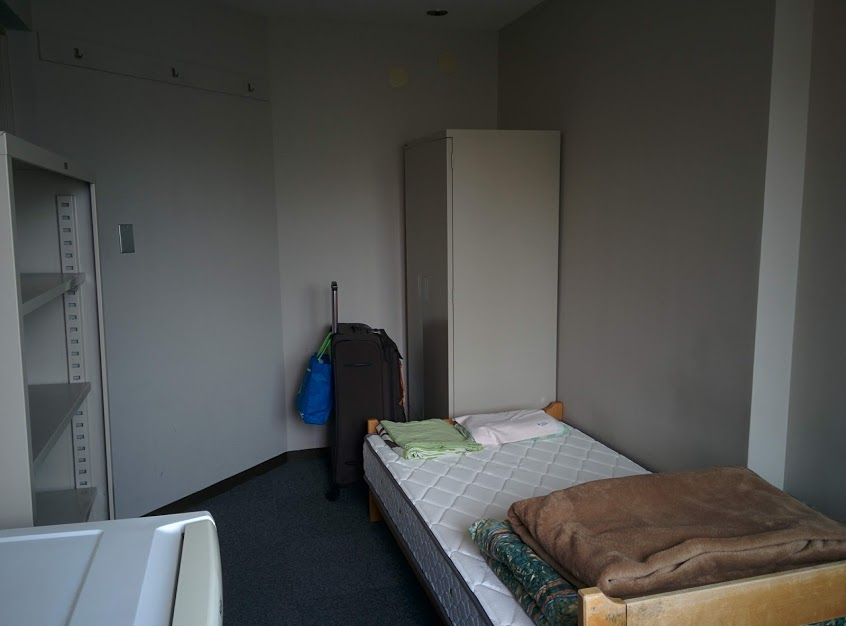
\includegraphics[width=0.45\linewidth]{dorm1}
    }
    \subfigure[ห้องนอน]{
        \label{Fig:dorm:2}
        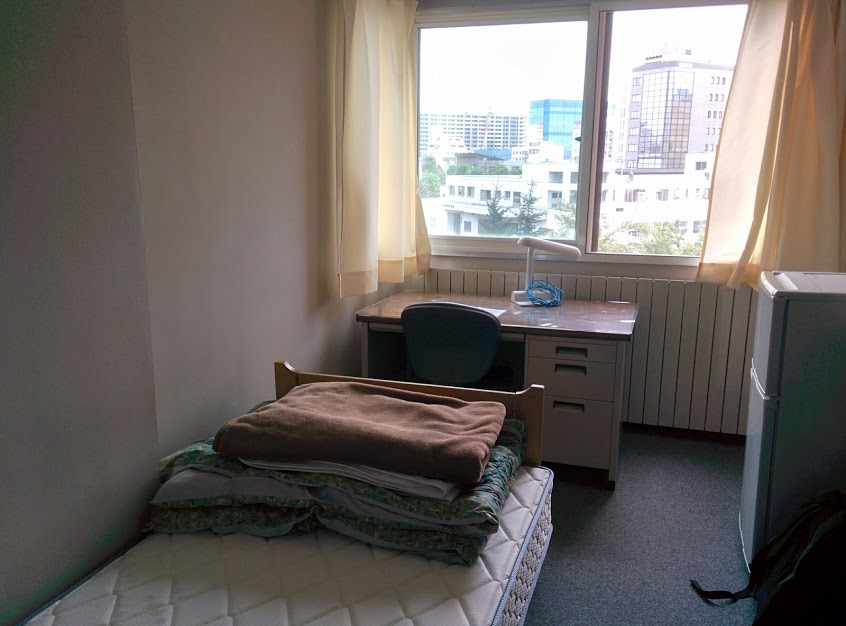
\includegraphics[width=0.45\linewidth]{dorm2}
    }
    \subfigure[ห้องอาหาร]{
        \label{Fig:dorm:3}
        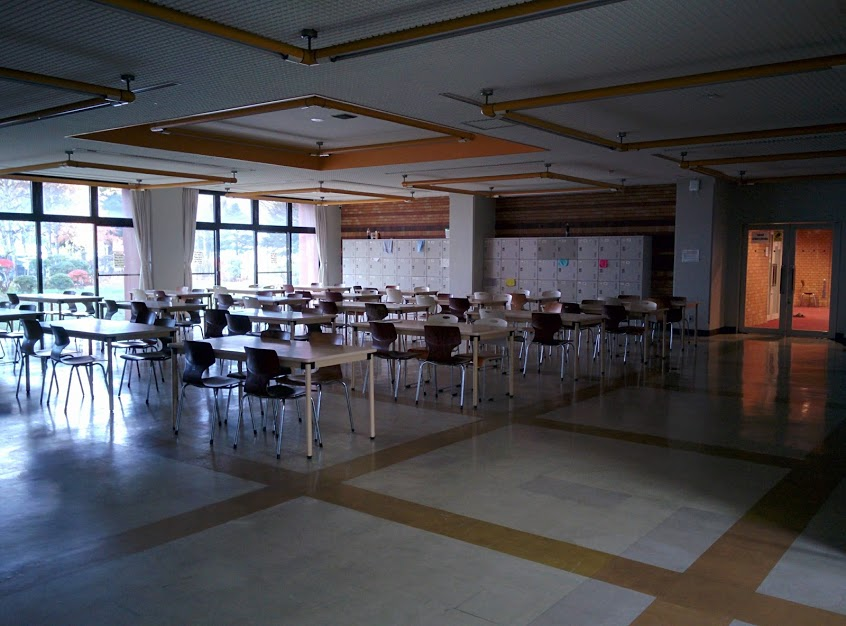
\includegraphics[width=0.45\linewidth]{dorm4}
    }
    \subfigure[ห้องครัว]{
        \label{Fig:dorm:4}
        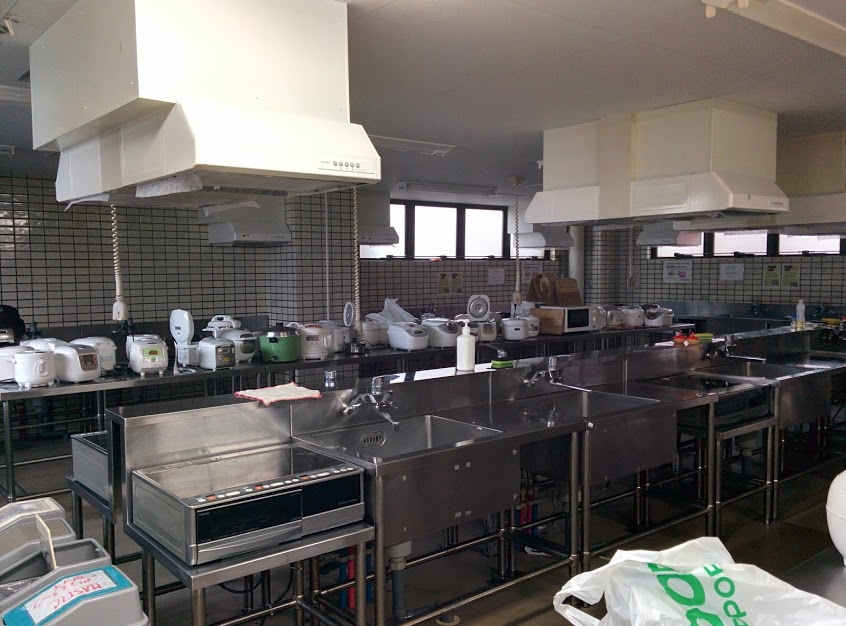
\includegraphics[width=0.45\linewidth]{dorm3}
    }
    \caption{ภาพหอพัก International House Kita 8 East}
    \label{Fig:dorm}
\end{figure}

\chapter{กิจกรรมระหว่างฝึกงาน}

นอกจากการมาทำโปรเจคแล้วนั้น ระหว่างสี่เดือนนี้ผมยังได้ร่วมกิจกรรมด้านวิชาการต่าง ๆ ดังเช่น การประชุมห้องทดลองรายสัปดาห์ และ การร่วมนำเสนอผลงานระหว่างห้องทดลอง เป็นต้น โดยรายละเอียดจะกล่าวต่อจากนี้

\section{Mirai Symposium}

กิจกรรมนี้จัดขึ้นที่เรียวกังหรือรีสอร์ทแบบญี่ปุ่น ซึ่งมีออนเซ็นหรือบ่อน้ำพุร้อนให้ได้แช่อีกด้วย ค่าใช้จ่ายทั้งหมดทางห้องทดลองออกให้ทั้งหมด ภายในงานจะมีกิจกรรมหลักคือการให้นักศึกษาทุกคนของห้องทดลองต่าง ๆ ที่มาร่วมงานนำผลงานตนเองมานำเสนอด้วยโปสเตอร์ในห้องประชุม หมุนเวียนไปเป็นช่วงเวลาคนละ 30 นาที หากสนใจงานของใครก็สามารถเดินไปสอบถามได้ อย่างที่เห็นในภาพ~\ref{Fig:mirai:1} การนำเสนอไม่ได้จำกัดว่างานต้องเป็นผลงานที่เสร็จสิ้นแล้ว อาจเป็นความก้าวหน้าของงานที่พัฒนาอยู่ได้เช่นเดียวกัน สำหรับครั้งนี้มีห้องทดลองร่วมงานสามห้องทดลอง สำหรับนักศึกษาต่างชาติจะมีนักศึกษาท่านอื่นเข้ามาสอบถามเพียงเล็กน้อยเนื่องจากต้องสื่อสารด้วยภาษาอังกฤษและนักศึกษาญี่ปุ่นส่วนใหญ่ไม่สามารถพูดอังกฤษได้ สำหรับงานวิจัยที่ผมพัฒนาก็ได้นำไปนำเสนอในงานนี้ด้วยเช่นเดียวกัน

เมื่อช่วงนำเสนอเสร็จสิ้น ทุกคนจะได้พักผ่อนตามอัธยาศัยโดยส่วนใหญ่จะเลือกไปแช่บ่อน้ำพุร้อนกัน สำหรับบ่อน้ำพุร้อนก็มีทั้งภายนอกและภายในอาคาร จากนั้นเป็นมื้อเย็นซึ่งเป็นอาหารชุดญี่ปุ่น~\ref{Fig:mirai:2}

\begin{figure}[!h]
    \centering
    \subfigure[บรรยากาศระหว่างการนำเสนอผลงานด้วยโปสเตอร์]{
        \label{Fig:mirai:1}
        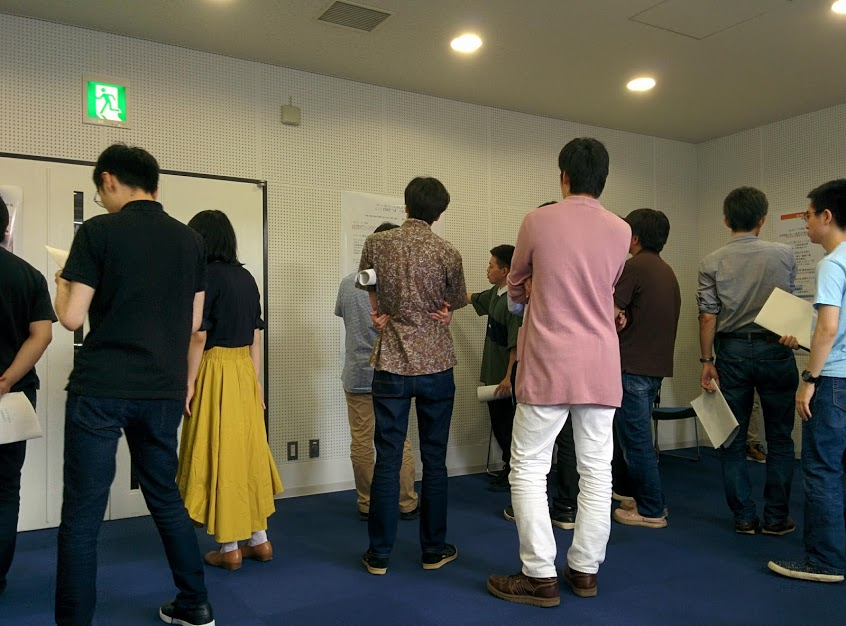
\includegraphics[width=0.8\linewidth]{mirai1}
    }
    \subfigure[ชุดอาหารจัดเลี้ยงมื้อเย็น]{
        \label{Fig:mirai:2}
        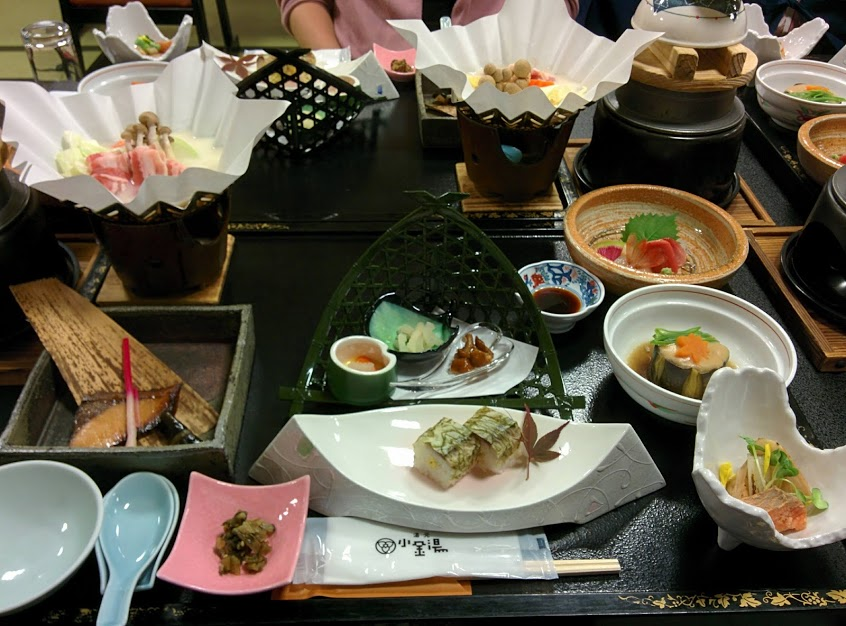
\includegraphics[width=0.45\linewidth]{mirai2}
    }
    \subfigure[ห้องอาหารจัดเลี้ยง]{
        \label{Fig:mirai:3}
        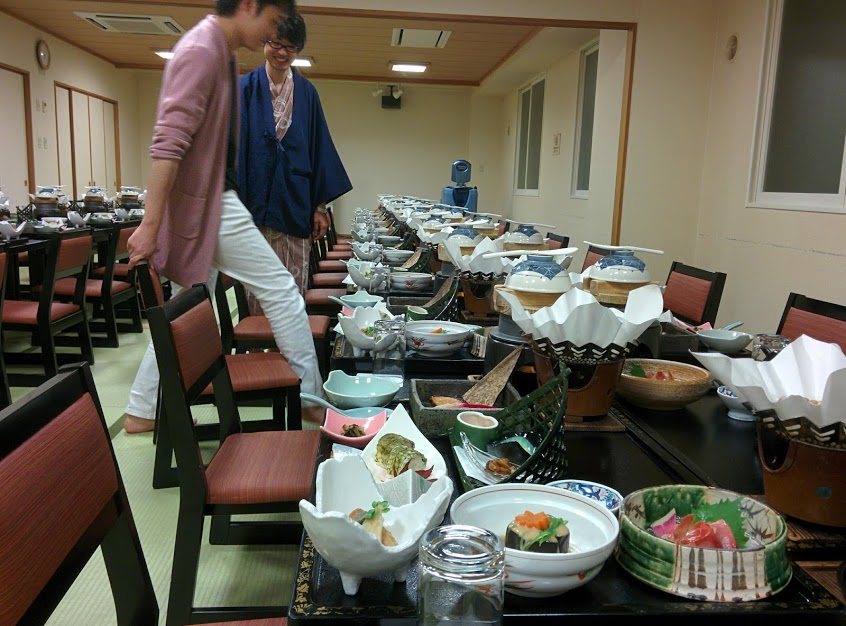
\includegraphics[width=0.45\linewidth]{mirai3}
    }
    \caption{ภาพกิจกรรมในงาน Mirai Symposium}
    \label{Fig:mirai}
\end{figure}

สำหรับวันที่สองก็มีกิจกรรมสร้างสรรค์ เป็นกิจกรรมที่ให้แยกกลุ่มกันและแก้โจทย์ปัญหาโดยให้แก้ภายในเวลาที่กำหนด ตัวอย่างคำถามเช่น \textit{มีเหรียญอยู่ร้อยเหรียญมีทั้งที่หงายหน้าก้อยและหัวอย่างละครึ่ง ต้องการแบ่งกลุ่มเหรียญสองกลุ่มโดยที่แต่ละกลุ่มมีจำนวนหน้าเหรียญและก้อยเท่า ๆ กัน โดยที่ผู้แบ่งมองไม่เห็นเหรียญจะทำได้อย่างไร} เป็นต้น เมื่อเสร็จกิจกรรมสร้างสรรค์ก็ถือเป็นการจบกิจกรรม Mirai Symposium แต่เพียงเท่านี้และเดินทางกลับมหาวิทยาลัย

\section{Lab Meeting}

สำหรับท้องทดลองที่ได้เข้ามาฝึกงานนั้นมีกิจกรรม Lab Meeting ทุกวันพุธ คือ กิจกรรมที่ให้สมาชิกภายในห้องทดลองร่วมกันนำงานวิจัยต่าง ๆ ที่ได้อ่านมานำเสนอต่อสมาชิกท่านอื่น ๆ ภายในห้องทดลอง โดยแต่ละสมาชิกจะถูกกำหนดวันเพื่อให้แต่ละคนที่ถูกกำหนดในวันนั้นนำ Conference Paper หรือ Journal ที่ถูกตีพิมพ์ในงานประชุมวิชาการชื่อดังของโลกมาร่วมกันนำเสนอแบบสรุปพร้อมสไลด์ กิจกรรมนี้ไม่มีคะแนนหรือรางวัลใด ๆ แต่เป็นการแลกเปลี่ยนความรู้ที่เกี่ยวข้องกับงานของตนเองที่ทำอยู่ 

สำหรับผมได้มีโอกาสนำเสนองานวิจัยที่ถูกตีพิมพ์ใน Journal เรื่อง \textit{Text-aware balloon extraction from manga} โดยหลังจากนำเสนอเสร็จสิ้นก็ได้รับคำถามและความคิดเห็นจากสมาชิกและอาจารย์ของห้องทดลองอย่างหลากหลาย ซึ่งถือเป็นโอกาสที่ดีในการเรียนรู้มุมมองและความคิดเห็นที่แปลกใหม่ต่องานของเรา

\section{กิจกรรมอื่น ๆ}

นอกจากกิจกรรมเชิงวิชาการแล้ว ผมยังได้ร่วมในกิจกรรมสังสรรค์อื่น ๆ เช่น งานเลี้ยงตามโอกาสต่าง ๆ โดยผมได้ร่วมงานเลี้ยงต้อนรับตัวผม ซึ่งจัดในช่วงเดือนตุลาคมที่ผ่านมา สาเหตุที่จัดช้าจากเดือนที่เข้าฝึกงานวันแรกไปหลายเดือนเนื่องจากกำหนดการในตอนแรกนั้นคือหนึ่งเดือนหลังจากผมมาอยู่ที่ประเทศญี่ปุ่น แต่ในช่วงกำหนดการเกิดเหตุการณ์แผ่นดินไหวใหญ่บนเกาะฮอกไกโดทำให้ต้องเลื่อนกำหนดการออกไป โดยงานเลี้ยงนี้จัดที่ร้านเนื้อย่างเจงกิสข่าน เป็นเนื้อแกะย่างบนเตาเหล็กลักษณะคล้ายหมูกระทะในประเทศไทยแตกต่างกันเพียงเน้นไปที่เนื้อแกะเป็นหลัก ภาพกิจกรรมแสดงในภาพ~\ref{Fig:welcome-party}

\begin{figure}[!h]
    \centering
    \subfigure[สมาชิกในห้องทดลองระหว่างกินเลี้ยง]{
        \label{Fig:welcome-party:1}
        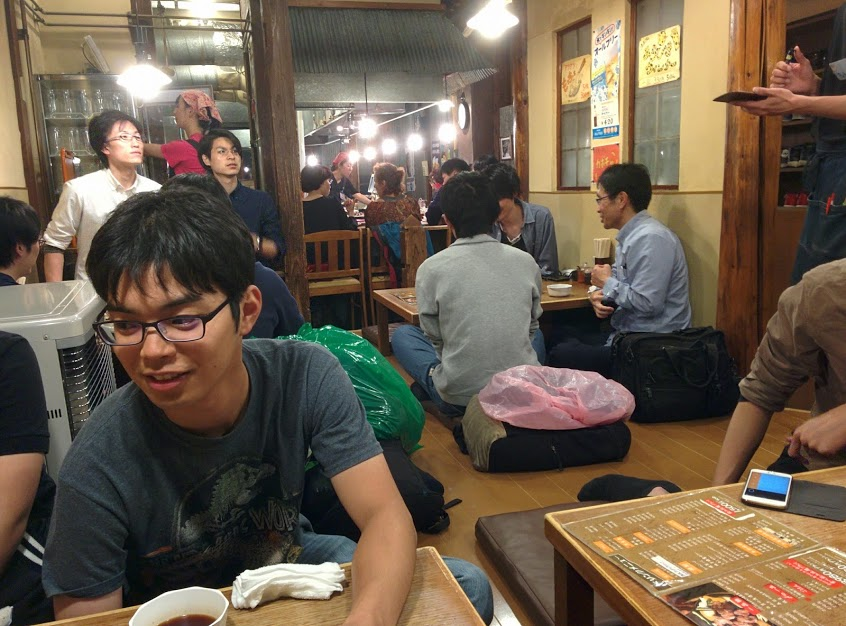
\includegraphics[width=0.8\linewidth]{welcome-party-1}
    }
    \subfigure[โต๊ะอาหารในร้านอาหารเจงกิสข่าน]{
        \label{Fig:welcome-party:2}
        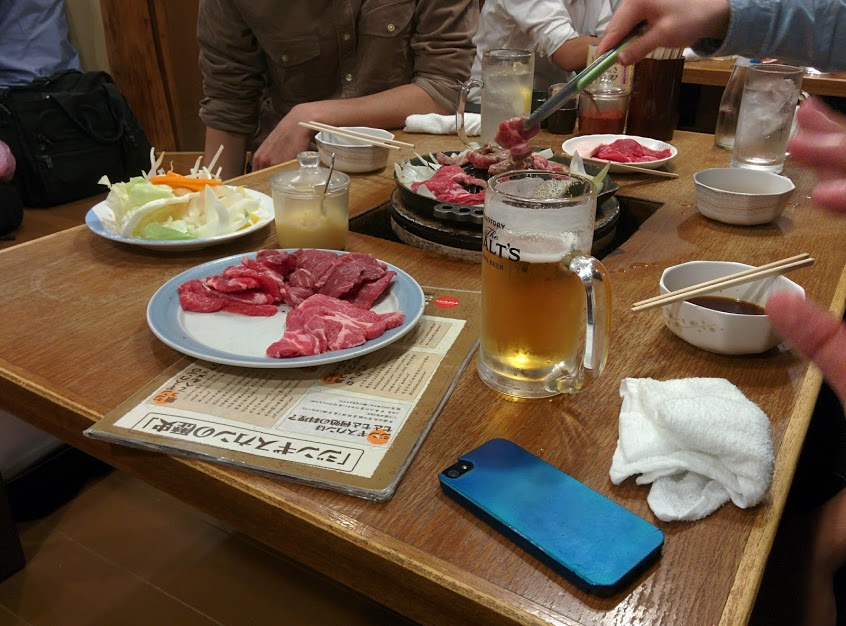
\includegraphics[width=0.45\linewidth]{welcome-party-2}
    }
    \subfigure[กระทะร้อนเจงกิสข่าน]{
        \label{Fig:welcome-party:3}
        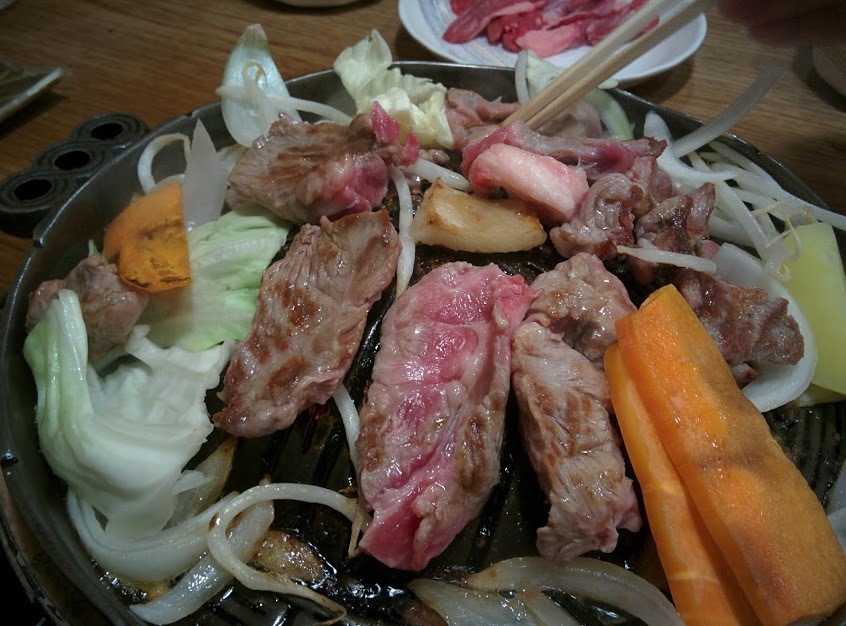
\includegraphics[width=0.45\linewidth]{welcome-party-3}
    }
    \caption{ภาพระหว่างงานเลี้ยงต้อนรับ}
    \label{Fig:welcome-party}
\end{figure}

นอกจากงานเลี้ยงต้อนรับแล้วยังมีงานเลี้ยงต้อนรับนักศึกษาปีสามที่เข้าเป็นสมาชิกใหม่ในห้องทดลองนี้อีกด้วย ซึ่งงานนี้จัดรวมเป็นงานเลี้ยงอำลาตัวผมพร้อม ๆ กันเนื่องจากจัดใกล้วันสิ้นสุดการฝึกงาน งานเลี้ยงจัดในห้องทดลองพร้อมด้วยอาหารหลากหลายชนิด งานไม่มีกิจกรรมอะไรมากมายเป็นเพียงการกินเลี้ยงเพื่อทำความรู้จักกับสมาชิกใหม่ของห้องทดลองและนั่งเล่นเกมด้วยกินตามที่แสดงในภาพ~\ref{Fig:farewell-party}

\begin{figure}[!h]
    \centering
    \subfigure[อาหารต่าง ๆ ในงานเลี้ยง]{
        \label{Fig:farewell:1}
        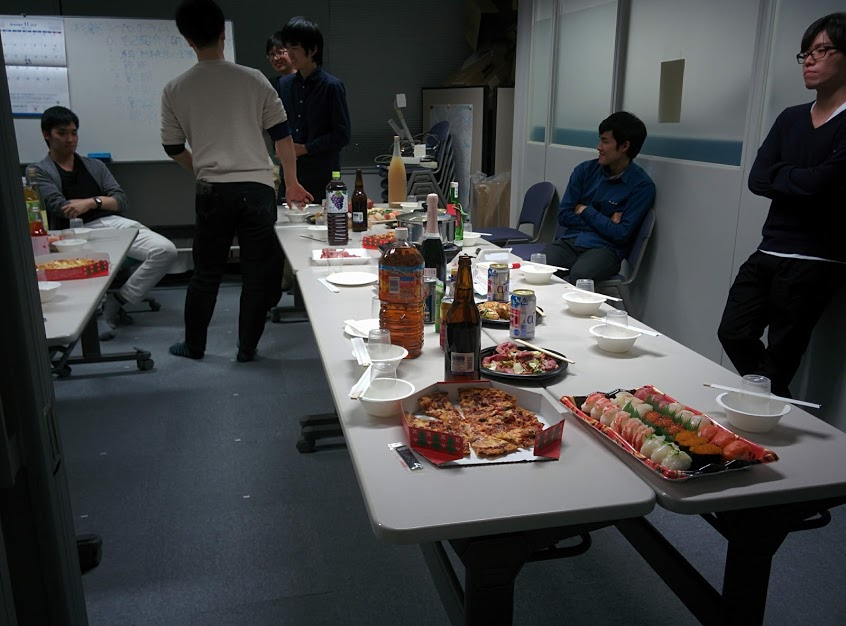
\includegraphics[width=0.8\linewidth]{farewell-party-1}
    }
    \subfigure[สมาชิกในห้องทดลองระหว่างเล่นเกมในงานเลี้ยง]{
        \label{Fig:farewell:2}
        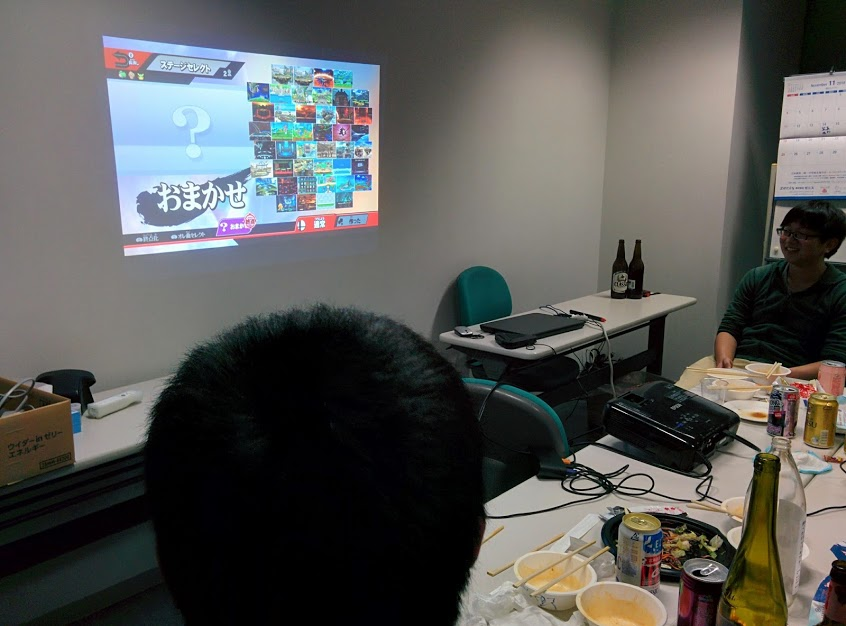
\includegraphics[width=0.8\linewidth]{farewell-party-2}
    }
    \caption{งานเลี้ยงอำลาและต้อนรับนักศึกษาปีสาม}
    \label{Fig:farewell-party}
\end{figure}

อธิบายเพิ่มเติมสำหรับงานเลี้ยงต้อนรับนักศึกษาปีสาม สำหรับห้องทดลองของคณะวิศวกรรมศาสตร์ที่ได้มาอยู่นี้จะมีการเปิดห้องทดลองให้นักศึกษาในคณะชั้นปีสามได้เข้าเยี่ยมชมห้องทดลองที่ตนเองสนใจก่อนจะเลือกเข้ามาเป็นสมาชิกในห้องทดลองที่เกี่ยวข้องกับงานที่สนใจจะทำ โดยงานที่สนใจจะทำจะกลายเป็นชิ้นงานจบการศึกษาคล้ายกับในมหาวิทยาลัยของไทย โดยในช่วงเวลานี้ของปีแต่ละห้องทดลองก็จะมีการโฆษณาห้องทดลองของตัวเองและเปิดโอกาสให้เข้าเยี่ยมชมงานภายในห้องทดลองว่าทำวิจัยเรื่องอะไร อย่างเช่นภาพ~\ref{Fig:ads} ที่เป็นป้ายเชิญเข้าชมห้องทดลองด้านเสียงและมีการใช้ตัวละครจากการ์ตูนเรื่อง Kemono Friend ประกอบให้น่าสนใจและดึงดูดมากขึ้น

\begin{figure}
    \centering
    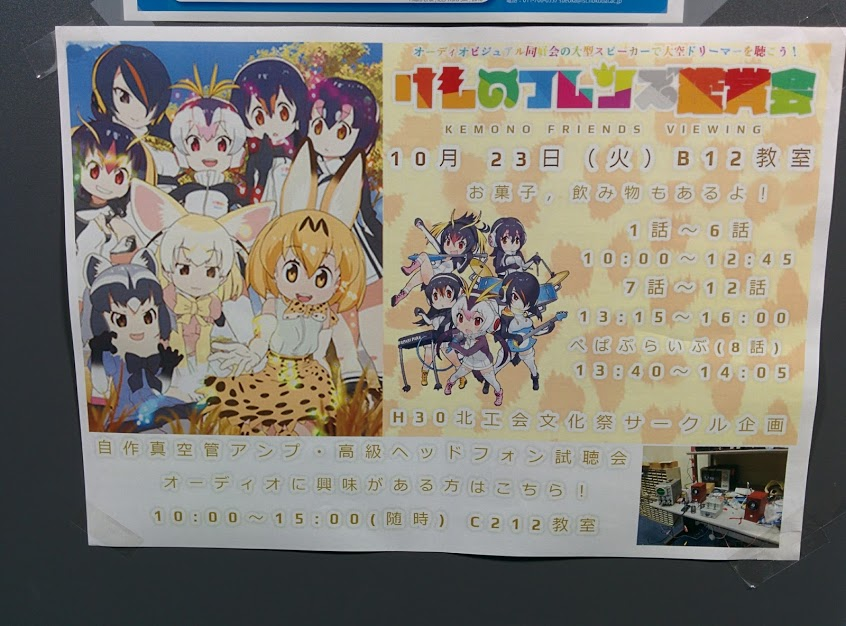
\includegraphics[width=0.8\linewidth]{ads}
    \caption{ป้ายเชิญชวนชมห้องทดลองโดยมีการใช้ตัวละครจากการ์ตูนประกอบให้น่าสนใจมากขึ้น}
    \label{Fig:ads}
\end{figure}

\clearpage 
\thispagestyle{empty}
\begin{center}
	\vspace*{\stretch{1}}
	\LARGE{\textbf{ภาคผนวก ค}}
	\vspace*{\stretch{1}}
\end{center}

\clearpage 
\thispagestyle{empty}
\begin{center}
    \vspace*{\stretch{1}}
    \LARGE{\textbf{ผลงานวิจัยที่ได้รับการตีพิมพ์}}
    \vspace*{\stretch{1}}
\end{center}

\addcontentsline{toc}{chapter}{ภาคผนวก\hspace{1ex}ค\hspace{2mm}ผลงานวิจัยที่ได้รับการตีพิมพ์}
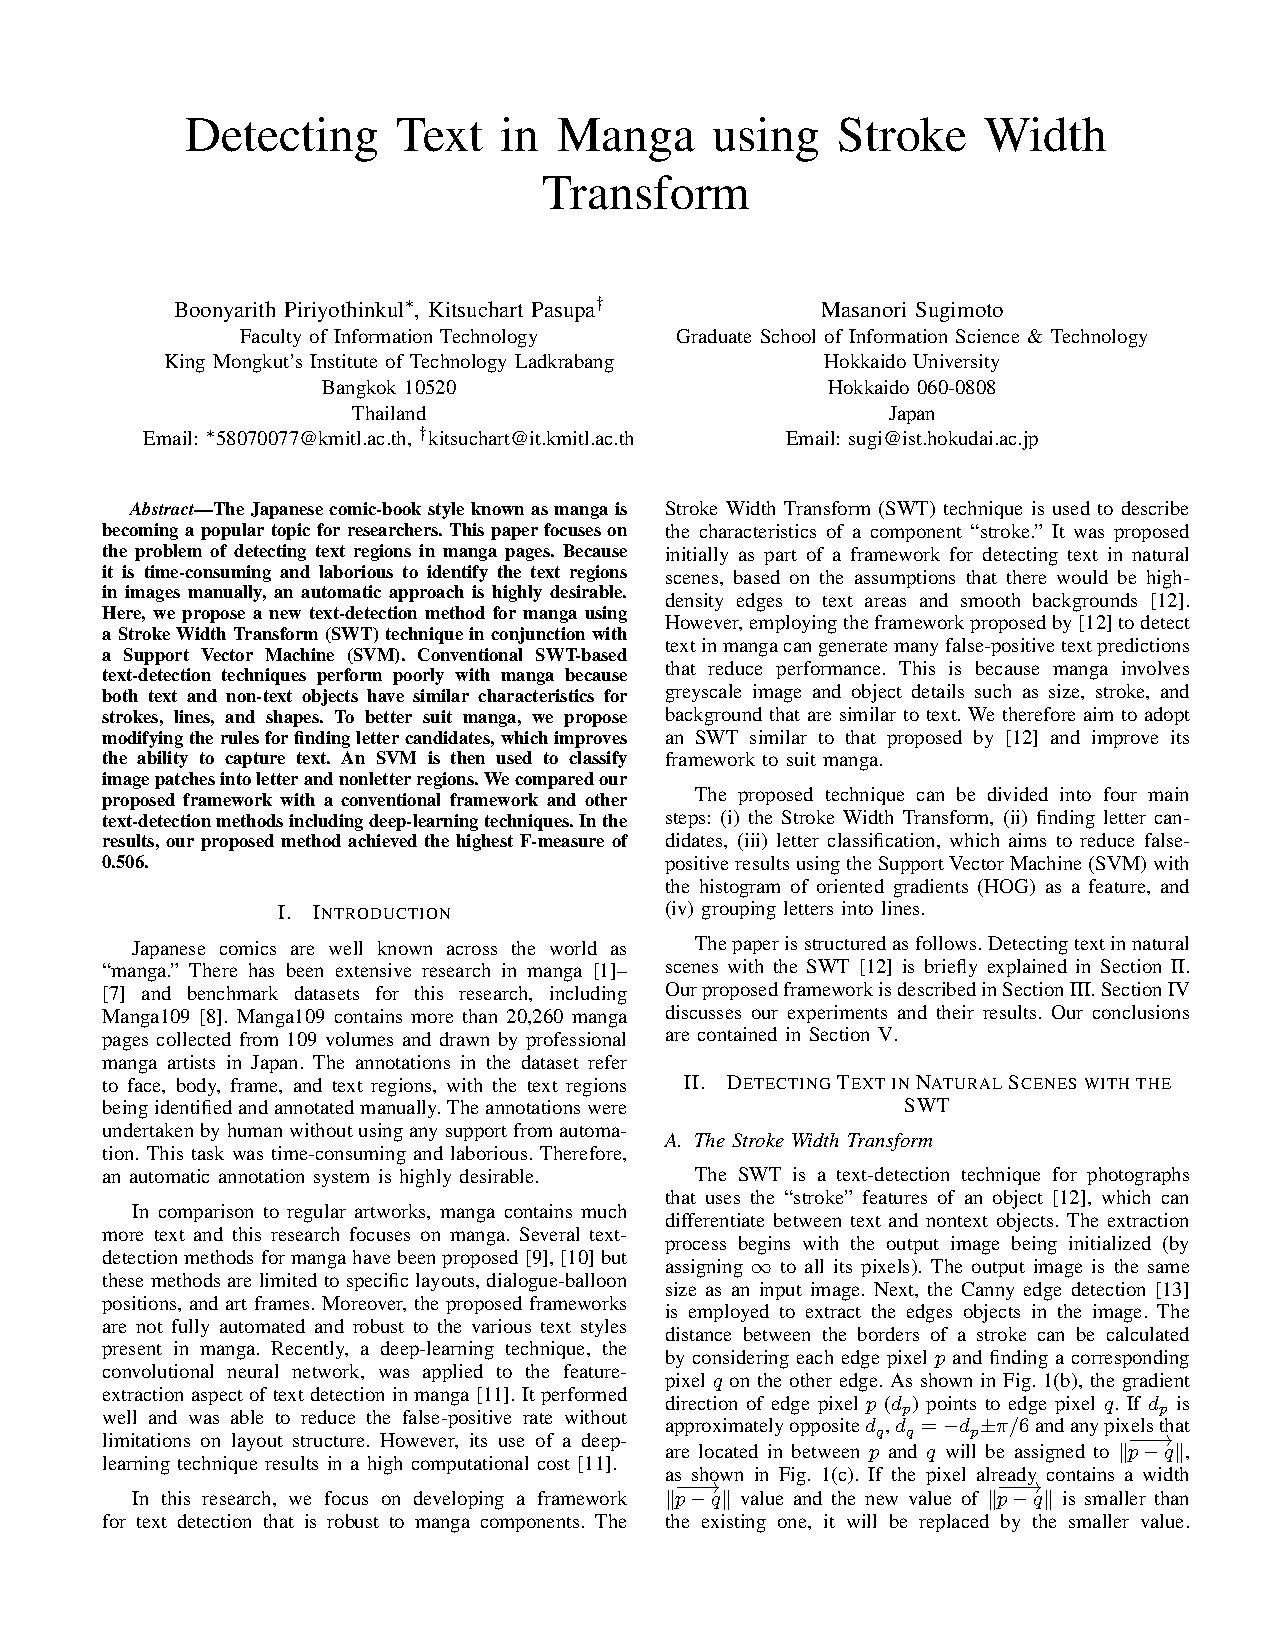
\includepdf[pages=-,pagecommand={}]{paper.pdf}

    \makeauthorbio

\end{document}
